% ============================================================
%  CHAPTER 16: HEAT TRANSFER
%  The Physics Codex: A Complete University Foundation
%  Korede Samuel Omotosho (Falcon)
%  Aurikrex Learning Systems, 2026
%
%  File: chapters/part2/ch16_heat_transfer.tex
% ============================================================

\chapter{Heat Transfer}
\label{ch:heat_transfer}
\minitoc
\newpage

\chapterquote{The sun, with all those planets revolving
around it and dependent upon it, can still ripen a
bunch of grapes as if it had nothing else in the
universe to do.}{Galileo Galilei}

\begin{objectivebox}
By the end of this chapter, you should be able to:
\begin{enumerate}[noitemsep]
  \item Describe and distinguish between conduction,
  convection and radiation as mechanisms of heat transfer
  \item Explain conduction in metals using the free
  electron model
  \item Apply Fourier's law of heat conduction
  quantitatively
  \item Explain natural and forced convection with
  real examples
  \item Describe the sea breeze and land breeze cycle
  \item State Stefan-Boltzmann Law and apply it to
  radiation problems
  \item Distinguish between black bodies, grey bodies
  and reflectors
  \item Explain the greenhouse effect and its
  relevance to climate
  \item Apply knowledge of all three mechanisms to
  practical problems including insulation
\end{enumerate}
\end{objectivebox}

% ============================================================
\section{Intuition: Three Ways Heat Travels}
% ============================================================

A metal rod with one end in a fire and one end in
your hand --- your hand gets hot. The heat travels
through the solid rod without any movement of the
rod itself. This is \textbf{conduction}.

Water in a pot on a stove --- the water at the bottom
heats up, becomes less dense, rises, and cold water
from the top sinks to replace it. The heat moves
because the water itself moves. This is
\textbf{convection}.

You stand near a bonfire and feel warmth on your
face, even though you are not touching anything and
no wind is blowing toward you. The heat travels as
invisible electromagnetic radiation through empty
space. This is \textbf{radiation}.

These three mechanisms are entirely different in
nature. Conduction requires physical contact and a
medium. Convection requires a fluid (liquid or gas)
that can move. Radiation requires neither contact
nor any medium --- it travels through a vacuum at
the speed of light.

Understanding all three is not merely academic.
Every building material, every cooking pot, every
roof sheet, every item of clothing, every cold store,
every solar panel --- all designed with these three
mechanisms in mind.

% ============================================================
\section{Conduction}
% ============================================================

\begin{definitionbox}[Thermal Conduction]
\textbf{Thermal conduction} is the transfer of heat
energy through a material by direct molecular
interaction, without any bulk movement of the material
itself. Heat flows from the hotter end to the cooler
end down the temperature gradient.
\end{definitionbox}

\subsection{Molecular Mechanism of Conduction}

\begin{diagbox}[Conduction: Molecular Vibration Chain in a Solid]
\begin{center}
\begin{tikzpicture}[scale=1.0, font=\small]

  % Rod
  \fill[gray!20] (0,0.5) rectangle (11,2.0);
  \draw[thick] (0,0.5) rectangle (11,2.0);

  % Hot end (left) - flames
  \fill[codexred!30] (-0.5,0.3) rectangle (0.5,2.2);
  \draw[codexred, very thick]
    (0,2.2) .. controls (-0.2,2.6) and (0.2,3.0)
    .. (0,3.3);
  \draw[codexred!70, thick]
    (-0.2,2.2) .. controls (-0.4,2.5) and (0.0,2.8)
    .. (-0.2,3.0);
  \draw[codexred!70, thick]
    (0.2,2.2) .. controls (0.4,2.5) and (0.0,2.8)
    .. (0.2,3.0);
  \node[codexred, font=\bfseries] at (0,-0.1)
    {Hot ($T_H$)};

  % Cold end (right) - ice blue
  \fill[codexblue!20] (10.5,0.3) rectangle (11.5,2.2);
  \draw[codexblue, very thick, dashed]
    (11,0.5) rectangle (11.5,2.0);
  \node[codexblue, font=\bfseries] at (11,-0.1)
    {Cold ($T_C$)};

  % Molecules along the rod (with vibration amplitude decreasing left to right)
  \foreach \x/\amp/\col in {
    1.0/0.45/codexred,
    2.2/0.38/codexred!80,
    3.4/0.31/codexred!60,
    4.6/0.25/codexgold!80,
    5.8/0.20/codexgold!60,
    7.0/0.15/codexblue!60,
    8.2/0.12/codexblue!70,
    9.4/0.09/codexblue!80} {
    % Molecule
    \fill[\col] (\x, 1.25) circle (7pt);
    % Vibration arc (shows amplitude)
    % Note: \col already carries tint information in the foreach list (e.g. codexred!80),
    % so adding another !80 would create an invalid xcolor expression like codexred!80!80.
    \draw[\col, thick]
      ({\x - \amp}, 1.25) -- ({\x + \amp}, 1.25);
    \draw[\col, thick, <->]
      ({\x - \amp}, 0.8) -- ({\x + \amp}, 0.8);
  }

  % Spring bonds between molecules
  \foreach \x in {1.0, 2.2, 3.4, 4.6, 5.8, 7.0, 8.2} {
    \draw[gray!50, thick, decorate,
      decoration={coil, amplitude=2pt, segment length=4pt}]
      (\x+0.07, 1.25) -- (\x+1.13, 1.25);
  }

  % Temperature gradient arrow
  \draw[->, very thick, codexgold]
    (1.0,-0.8) -- (9.5,-0.8)
    node[right, font=\small]{Heat flow (from hot to cold)};

  % Amplitude labels
  \node[codexred, font=\tiny, align=center] at (1.0, 0.55)
    {Large\\vibration};
  \node[codexblue, font=\tiny, align=center] at (9.4, 0.55)
    {Small\\vibration};

  % Temperature gradient curve
  \draw[codexgold, dashed, thick]
    (1.0,2.3) .. controls (3,2.1) and (7,1.7) .. (9.4,1.5);
  \node[codexgold, font=\tiny] at (5,2.3)
    {Temperature decreases along rod};

\end{tikzpicture}
\end{center}
\small Hot end molecules vibrate vigorously. They
collide with neighbours, transferring energy along
the chain. Vibration amplitude decreases from hot
end to cold end. In metals, free electrons also carry
energy much faster than lattice vibrations.
\end{diagbox}

\begin{keybox}[Why Metals Conduct Better Than Non-Metals]
In metals, there are free electrons that move
throughout the material. When the hot end is heated,
these electrons gain kinetic energy and diffuse
rapidly toward the cooler end, colliding with lattice
ions and transferring energy. This \textit{electron
conduction} is much faster than the slower
vibration-to-vibration (phonon) mechanism in
non-metals. This is why metals feel cold to the
touch even at room temperature --- they conduct heat
away from your fingers rapidly.

Materials like wood, rubber, glass, and still air
are poor conductors (good insulators) because they
lack free electrons.
\end{keybox}

\begin{table}[H]
\centering
\caption{Thermal Conductivities of Common Materials}
\label{tab:conductivity}
\begin{tabular}{ll}
\toprule
\textbf{Material} & \textbf{Thermal Conductivity $k$
(W\,m$^{-1}$\,K$^{-1}$)}\\
\midrule
Silver & 429\\
Copper & 385\\
Aluminium & 205\\
Steel (mild) & 50\\
Glass & 1.0\\
Concrete & 0.8--1.4\\
Brick & 0.6--1.0\\
Water & 0.60\\
Wood (dry) & 0.10--0.15\\
Still air & 0.025\\
Wool/fibreglass insulation & 0.04\\
\bottomrule
\end{tabular}
\end{table}

\subsection{Fourier's Law of Heat Conduction}

\begin{lawbox}[Fourier's Law of Heat Conduction]
The rate of heat flow through a slab of material is:
\[
  \frac{dQ}{dt} = kA\frac{\Delta T}{L}
  = kA\frac{(T_H - T_C)}{L}
\]
where:
\begin{itemize}[noitemsep]
  \item $dQ/dt$ = rate of heat flow (W)
  \item $k$ = thermal conductivity
  (W\,m$^{-1}$\,K$^{-1}$)
  \item $A$ = cross-sectional area (m$^2$)
  \item $\Delta T = T_H - T_C$ = temperature
  difference (K)
  \item $L$ = thickness of slab (m)
\end{itemize}
\[
  \frac{\Delta T}{L} = \text{temperature gradient
  (K\,m}^{-1}\text{)}
\]
\end{lawbox}

\begin{diagbox}[Fourier's Law: Heat Flow Through a Slab]
\begin{center}
\begin{tikzpicture}[scale=1.0, font=\small]

  % Slab
  \fill[gray!25] (3,0) rectangle (6,5);
  \draw[very thick] (3,0) rectangle (6,5);

  % Hot side
  \fill[codexred!20] (0,0) rectangle (3,5);
  \draw[codexred, very thick] (3,0) -- (3,5);
  \node[codexred, font=\bfseries, align=center] at (1.5,2.5)
    {Hot side\\$T_H$};

  % Cold side
  \fill[codexblue!15] (6,0) rectangle (9,5);
  \draw[codexblue, very thick] (6,0) -- (6,5);
  \node[codexblue, font=\bfseries, align=center] at (7.5,2.5)
    {Cold side\\$T_C$};

  % Heat flow arrows through slab
  \foreach \y in {0.7,1.5,2.5,3.5,4.3} {
    \draw[->, very thick, codexgold]
      (3.2,\y) -- (5.8,\y);
  };

  % Thickness label
  \draw[<->, gray, thick] (3,-0.4) -- (6,-0.4);
  \node[below, gray] at (4.5,-0.5) {$L$ (thickness)};

  % Area label
  \draw[<->, gray, thick] (9.5,0) -- (9.5,5);
  \node[right, gray] at (9.6,2.5) {$A$ (area)};

  % Formula
  \node[align=center, font=\normalsize, codexgold]
    at (4.5,6.0)
    {Heat flow $\dfrac{dQ}{dt} = kA\dfrac{T_H - T_C}{L}$};

  % Temperature gradient inside slab
  \draw[codexgold, very thick, dashed]
    (3,4.5) -- (6,1.2);
  \node[codexgold, font=\scriptsize, align=center,
    fill=white, inner sep=1pt]
    at (4.5,4.65) {$\Delta T/L$ (gradient)};

\end{tikzpicture}
\end{center}
\end{diagbox}

\begin{examplebox}[16.1]
\stepcounter{workedexample}
A glass window pane is $4.0\ \text{mm}$ thick and
$1.5\ \text{m} \times 1.2\ \text{m}$ in area. The
inside temperature is $22°\text{C}$ and the outside
temperature is $5°\text{C}$.\\
($k_{glass} = 1.0\ \text{W\,m}^{-1}\text{K}^{-1}$)\\
(a) Calculate the rate of heat loss through the
window.\\
(b) How much heat is lost in 8 hours?\\
(c) Why is double glazing effective?
\end{examplebox}

\begin{solutionbox}
$A = 1.5 \times 1.2 = 1.8\ \text{m}^2$,
$L = 4.0\times10^{-3}\ \text{m}$,
$\Delta T = 22 - 5 = 17\ \text{K}$

\textbf{(a)} Rate of heat loss:
\[
  \frac{dQ}{dt} = kA\frac{\Delta T}{L}
  = 1.0 \times 1.8 \times \frac{17}{4.0\times10^{-3}}
  = 1.8 \times 4250
  = 7650\ \text{W}
\]

\textbf{(b)} In 8 hours ($t = 8 \times 3600
= 28\,800\ \text{s}$):
\[
  Q = \frac{dQ}{dt} \times t
  = 7650 \times 28\,800
  = 2.20\times10^8\ \text{J} \approx 220\ \text{MJ}
\]

\textbf{(c)} Double glazing has two panes of glass
with a layer of still air (or inert gas) between them.
Still air has $k \approx 0.025\ \text{W\,m}^{-1}\text{K}^{-1}$
--- about 40 times lower than glass. The trapped air
layer dramatically reduces the temperature gradient
across the glass and thus the rate of heat flow.
The glass panes themselves contribute little to
the insulation; all the benefit comes from the
trapped still air.
\end{solutionbox}

\begin{examplebox}[16.2]
\stepcounter{workedexample}
A composite wall consists of a $20\ \text{cm}$ thick
brick layer ($k = 0.80\ \text{W\,m}^{-1}\text{K}^{-1}$)
and a $5\ \text{cm}$ thick insulation board
($k = 0.040\ \text{W\,m}^{-1}\text{K}^{-1}$).
The inner surface is at $18°\text{C}$ and the outer
surface at $-2°\text{C}$. The wall area is $10\ \text{m}^2$.\\
Find the rate of heat loss through the wall.
\end{examplebox}

\begin{solutionbox}
For layers in series, the same heat flow passes
through each layer. Define \textbf{thermal resistance}:
\[
  R = \frac{L}{kA}
  \quad (\text{analogous to electrical resistance})
\]

$R_{brick} = \frac{0.20}{0.80 \times 10}
= \frac{0.20}{8.0} = 0.025\ \text{K\,W}^{-1}$

$R_{insulation} = \frac{0.05}{0.040 \times 10}
= \frac{0.05}{0.40} = 0.125\ \text{K\,W}^{-1}$

$R_{total} = 0.025 + 0.125 = 0.150\ \text{K\,W}^{-1}$

Rate of heat loss:
\[
  \frac{dQ}{dt} = \frac{\Delta T}{R_{total}}
  = \frac{18 - (-2)}{0.150}
  = \frac{20}{0.150}
  = 133\ \text{W}
\]

The insulation layer contributes $0.125/0.150
= 83\%$ of the total thermal resistance despite
being only $5\ \text{cm}$ thick. The thin insulation
board does five times more work than the $20\ \text{cm}$
brick wall it is protecting.
\end{solutionbox}

% ============================================================
\section{Convection}
% ============================================================

\begin{definitionbox}[Convection]
\textbf{Convection} is the transfer of heat energy
through a fluid (liquid or gas) by the bulk movement
of the fluid itself. Hot fluid expands, becomes less
dense, rises, and is replaced by cooler, denser fluid.
This sets up a \textbf{convection current}.

\textbf{Natural (free) convection:} Driven by density
differences due to temperature.

\textbf{Forced convection:} A pump or fan forces
the fluid to move (e.g.\ central heating systems,
car radiator fans, air conditioners).
\end{definitionbox}

\begin{diagbox}[Natural Convection Loop in a Liquid]
\begin{center}
\begin{tikzpicture}[scale=1.0, font=\small]

  % Container
  \fill[codexblue!10] (-0.5,-0.5) rectangle (7.5,6.0);
  \draw[very thick] (-0.5,-0.5) rectangle (7.5,6.0);

  % Heat source (bottom left)
  \fill[codexred!40] (0.3,0) rectangle (2.0,0.4);
  \draw[codexred, very thick]
    (0.3,0.4) -- (2.0,0.4);
  \node[codexred, font=\small] at (1.15,-0.3)
    {Heat source};

  % Convection current arrows (main loop)
  % Rising hot fluid (left side)
  \draw[->, very thick, codexred, line width=2pt]
    (1.0,0.5) -- (1.0,5.0);
  \draw[->, very thick, codexred!70, line width=1.5pt]
    (1.0,5.0) -- (4.0,5.0);
  \draw[->, very thick, codexblue, line width=1.5pt]
    (4.0,5.0) -- (6.0,5.0);
  % Sinking cool fluid (right side)
  \draw[->, very thick, codexblue, line width=2pt]
    (6.0,5.0) -- (6.0,0.5);
  \draw[->, very thick, codexblue!70, line width=1.5pt]
    (6.0,0.5) -- (3.5,0.5);
  \draw[->, very thick, codexblue!50, line width=1.5pt]
    (3.5,0.5) -- (1.0,0.5);

  % Secondary loop arrows
  \draw[->, thick, codexred!50]
    (2.5,0.5) -- (2.5,4.0);
  \draw[->, thick, codexblue!50]
    (5.0,4.5) -- (5.0,0.5);

  % Temperature labels
  \node[codexred, font=\small, align=center] at (0.3,3.0)
    {Hot\\rises};
  \node[codexblue, font=\small, align=center] at (6.5,3.0)
    {Cool\\sinks};
  \node[codexred!70, font=\small] at (3.5,5.3)
    {Hot fluid spreads at top};
  \node[codexblue!70, font=\small] at (4.5,-0.05)
    {Cool fluid returns};

  % Molecule density illustration
  \node[align=center, font=\tiny] at (1.5,2.5)
    {Less\\dense\\(hot)};
  \node[align=center, font=\tiny] at (5.5,2.5)
    {More\\dense\\(cool)};

  % Label
  \node[font=\small, align=center] at (3.5,-1.4)
    {Natural convection loop: hot fluid rises, cool fluid sinks,\\
    setting up a continuous circulation current};

\end{tikzpicture}
\end{center}
\end{diagbox}

\subsection{The Sea Breeze and Land Breeze}

The sea breeze and land breeze are direct consequences
of convection driven by the different thermal properties
of land and sea. Land has a much lower specific heat
capacity than seawater, so land heats up and cools
down much faster than the sea for the same solar input.

\begin{diagbox}[Sea Breeze (Daytime) and Land Breeze (Night-time)]
\begin{center}
\begin{tikzpicture}[font=\small]
  % === DAY: SEA BREEZE === (panel width 5.5, height ~5.9)
  \begin{scope}[shift={(0,0)}]
    \node[font=\bfseries\small, codexgold] at (2.75,5.6) {DAY: Sea Breeze};
    % Sun
    \fill[codexgold] (4.6,5.0) circle (0.35);
    \foreach \angle in {0,30,...,330} {
      \draw[codexgold, thick]
        ({4.6+0.42*cos(\angle)},{5.0+0.42*sin(\angle)})
        -- ({4.6+0.58*cos(\angle)},{5.0+0.58*sin(\angle)});
    }
    % Land (left, hot)
    \fill[brown!40] (0,0) rectangle (2.75,0.8);
    \draw[thick] (0,0.8) -- (2.75,0.8);
    \node[brown!60, font=\tiny] at (1.375,0.4) {Land (hot, low $c$)};
    % Sea (right, cooler)
    \fill[codexblue!30] (2.75,0) rectangle (5.5,0.8);
    \draw[thick] (2.75,0.8) -- (5.5,0.8);
    \node[codexblue!80, font=\tiny] at (4.125,0.4) {Sea (cool, high $c$)};
    % Dividing line
    \draw[thick, dashed] (2.75,0) -- (2.75,5.3);
    % Hot air rises over land, flows to sea, descends
    \draw[->, very thick, codexred, line width=1.6pt] (1.375,0.8) -- (1.375,4.0);
    \draw[->, very thick, codexred!70, line width=1.2pt] (1.375,4.0) -- (4.125,4.0);
    \draw[->, very thick, codexblue, line width=1.6pt] (4.125,4.0) -- (4.125,0.95);
    % Low-level flow: sea to land (the SEA BREEZE)
    \draw[->, very thick, codexblue, line width=2pt] (3.5,1.05) -- (1.9,1.05);
    \node[codexblue, font=\small, align=center] at (2.8,1.6) {Sea breeze };
    % Heat waves over land
    \foreach \x in {0.6,1.1,1.6,2.1} {
      \draw[codexred, thin] (\x,0.8) .. controls (\x-0.07,1.0) and (\x+0.07,1.2) .. (\x,1.4);
    }
    % Labels
    \node[codexred, font=\tiny, align=center] at (0.85,2.6) {Hot air\\rises};
    \node[codexblue, font=\tiny, align=center] at (4.55,2.6) {Cool air\\descends};
  \end{scope}
  % === NIGHT: LAND BREEZE === (shifted by panel width + gap)
  \begin{scope}[shift={(6.3,0)}]
    \node[font=\bfseries\small, codexblue] at (2.75,5.6) {NIGHT: Land Breeze};
    % Moon
    \fill[gray!60] (4.6,5.0) circle (0.4);
    \fill[gray!20] (4.6,5.0) circle (0.3);
    % Land (left, now cold)
    \fill[gray!40] (0,0) rectangle (2.75,0.8);
    \draw[thick] (0,0.8) -- (2.75,0.8);
    \node[gray!80, font=\tiny] at (1.375,0.4) {Land (cold, cools fast)};
    % Sea (right, warmer at night)
    \fill[codexblue!40] (2.75,0) rectangle (5.5,0.8);
    \draw[thick] (2.75,0.8) -- (5.5,0.8);
    \node[codexblue, font=\tiny] at (4.125,0.4) {Sea (warmer at night)};
    % Dividing line
    \draw[thick, dashed] (2.75,0) -- (2.75,5.3);
    % Warm air rises over sea, flows to land, descends
    \draw[->, very thick, codexred, line width=1.6pt] (4.125,0.8) -- (4.125,4.0);
    \draw[->, very thick, codexred!70, line width=1.2pt] (4.125,4.0) -- (1.375,4.0);
    \draw[->, very thick, codexblue, line width=1.6pt] (1.375,4.0) -- (1.375,0.95);
    % Low-level flow: land to sea (the LAND BREEZE)
    \draw[->, very thick, codexblue!80, line width=2pt] (2.0,1.05) -- (3.6,1.05);
    \node[codexblue!80, font=\small, align=center] at (2.7,1.6) {Land breeze};
    % Labels
    \node[codexred, font=\tiny, align=center] at (4.85,2.6) {Warm air\\rises};
    \node[codexblue, font=\tiny, align=center] at (0.65,2.6) {Cool air\\descends};
  \end{scope}
\end{tikzpicture}
\end{center}
\small Fishermen along the coasts of Nigeria, Ghana and
Côte d'Ivoire have relied on sea breezes and land
breezes for centuries to navigate their boats --- out
to sea in the morning with the land breeze, returning
in the afternoon with the sea breeze.
\end{diagbox}

% ============================================================
\section{Radiation}
% ============================================================

\begin{definitionbox}[Thermal Radiation]
\textbf{Thermal radiation} is the emission of energy
in the form of electromagnetic waves (infrared
radiation) by all objects with temperature above
absolute zero. It requires no medium --- it travels
through vacuum at the speed of light
($3\times10^8\ \text{m\,s}^{-1}$).

All objects simultaneously \textit{emit} and
\textit{absorb} radiation. The net heat transfer
is from the hotter to the cooler object.
\end{definitionbox}

\begin{diagbox}[Good and Poor Emitters/Absorbers of Radiation]
\begin{center}
\begin{tikzpicture}[scale=1.0, font=\small]

  % === BLACK SURFACE ===
  \begin{scope}[shift={(0,3.0)}]
    \node[font=\bfseries] at (2.5,2.5)
      {Black (Matt) Surface};

    % Object
    \fill[black!80] (1.0,0) rectangle (4.0,1.5);
    \draw[thick] (1.0,0) rectangle (4.0,1.5);
    \node[white, font=\small] at (2.5,0.75)
      {Black surface};

    % Many emission arrows (lots of radiation)
    \foreach \x in {1.3,1.8,2.3,2.8,3.3,3.7} {
      \draw[->, thick, codexred]
        (\x,1.5) -- (\x+0.2, 2.3);
    }
    \foreach \x in {1.5,2.0,2.5,3.0,3.5} {
      \draw[->, thick, codexred]
        (\x,1.5) -- (\x-0.2, 2.3);
    }
    \node[codexred, font=\small] at (2.5,3.1)
      {Strong emission};

    % Many absorption arrows
    \foreach \x in {1.4,1.9,2.4,2.9,3.4} {
      \draw[<-, thick, codexgold]
        (\x,0) -- (\x+0.1,-0.6);
    }
    \node[codexgold, font=\small] at (2.5,-1.0)
      {Strong absorption};
    \node[font=\small, align=center] at (2.5,-2.0)
      {Absorbs and emits\\most radiation};
  \end{scope}

  % === SHINY SURFACE ===
  \begin{scope}[shift={(6.0,3.0)}]
    \node[font=\bfseries] at (2.5,2.5)
      {Shiny (Polished) Surface};

    % Object
    \fill[gray!20] (1.0,0) rectangle (4.0,1.5);
    \fill[white] (1.05,0.05) rectangle (3.95,1.45);
    \draw[thick] (1.0,0) rectangle (4.0,1.5);
    % Shine lines
    \foreach \y in {0.3,0.7,1.1} {
      \draw[gray!60] (1.1,\y) -- (2.0,\y);
    }
    \node[font=\small] at (2.5,0.75)
      {Polished metal};

    % Few emission arrows
    \draw[->, thick, codexred!50]
      (2.0,1.5) -- (2.2,2.3);
    \draw[->, thick, codexred!50]
      (3.0,1.5) -- (2.8,2.3);
    \node[codexred!60, font=\small] at (2.5,3.1)
      {Weak emission};

    % Reflection arrows (incoming radiation reflected)
    \draw[->, thick, codexgold]
      (1.5,-0.7) -- (1.5,0);
    \draw[->, thick, codexgold, dashed]
      (1.5,0) -- (0.8,-0.5);
    \draw[->, thick, codexgold]
      (3.5,-0.7) -- (3.5,0);
    \draw[->, thick, codexgold, dashed]
      (3.5,0) -- (4.2,-0.5);
    \node[codexgold, font=\small] at (2.5,-1.0)
      {Mostly reflects};
    \node[font=\small, align=center] at (2.5,-2.0)
      {Reflects most radiation,\\absorbs/emits little};
  \end{scope}

  % Summary rule
  \node[codexblue, font=\small, align=center]
    at (5.5,-0.3)
    {\textbf{Good absorbers are good emitters}\\
    \textbf{Poor absorbers are poor emitters}\\
    (This is Kirchhoff's Law of Radiation)};

\end{tikzpicture}
\end{center}
\end{diagbox}

\subsection{Factors Affecting Radiation}

The rate of emission of thermal radiation by an
object depends on:
\begin{enumerate}[noitemsep]
  \item \textbf{Temperature} of the surface
  (very strongly --- as $T^4$)
  \item \textbf{Surface area} (proportional to area)
  \item \textbf{Nature of the surface} (black/matt
  surfaces emit more than shiny/polished surfaces)
  \item \textbf{Colour} (dark colours absorb and emit
  more than light colours)
\end{enumerate}

\begin{lawbox}[Stefan-Boltzmann Law]
The power radiated per unit area by a perfect emitter
(black body) at absolute temperature $T$ is:
\[
  \frac{P}{A} = \sigma T^4
\]
Total power radiated:
\[
  P = \sigma A T^4
\]
where $\sigma = 5.67\times10^{-8}\ \text{W\,m}^{-2}\text{K}^{-4}$
is the Stefan-Boltzmann constant.

For a grey body (real surface) with emissivity
$\varepsilon$ ($0 < \varepsilon \leq 1$):
\[
  P = \varepsilon\sigma A T^4
\]
For a black body (perfect emitter): $\varepsilon = 1$.
For a polished metal surface: $\varepsilon \approx 0.05$.

\textbf{Net power radiated} by an object at
temperature $T$ in surroundings at temperature
$T_0$:
\[
  P_{net} = \varepsilon\sigma A(T^4 - T_0^4)
\]
\end{lawbox}

\begin{examplebox}[16.3]
\stepcounter{workedexample}
The surface of the Sun has temperature
$5778\ \text{K}$ and radius $6.96\times10^8\ \text{m}$.
Treating it as a black body:
($\sigma = 5.67\times10^{-8}\ \text{W\,m}^{-2}\text{K}^{-4}$)\\
(a) Calculate the total power radiated by the Sun.\\
(b) Calculate the solar intensity at Earth's
distance ($d = 1.50\times10^{11}\ \text{m}$ from
the Sun).\\
(c) The Earth absorbs $\approx 70\%$ of the solar
radiation hitting it. What equilibrium temperature
would Earth have if it radiated as a black body with
effective area equal to its cross-sectional area
($r_E = 6.37\times10^6\ \text{m}$)?
\end{examplebox}

\begin{solutionbox}
\textbf{(a)} Surface area of Sun:
$A_{Sun} = 4\pi r_{Sun}^2
= 4\pi(6.96\times10^8)^2
= 6.087\times10^{18}\ \text{m}^2$

Total power:
\[
  P_{Sun} = \sigma A_{Sun} T^4
  = 5.67\times10^{-8} \times 6.087\times10^{18}
  \times 5778^4
\]
\[
  = 5.67\times10^{-8} \times 6.087\times10^{18}
  \times 1.116\times10^{15}
  = 3.85\times10^{26}\ \text{W}
\]

\textbf{(b)} Solar intensity at Earth (intensity
spread over sphere of radius $d$):
\[
  I = \frac{P_{Sun}}{4\pi d^2}
  = \frac{3.85\times10^{26}}
    {4\pi(1.50\times10^{11})^2}
  = \frac{3.85\times10^{26}}
    {2.827\times10^{23}}
  = 1362\ \text{W\,m}^{-2}
\]
This is the \textbf{solar constant}. The accepted
value is $1361\ \text{W\,m}^{-2}$ --- excellent
agreement.

\textbf{(c)} Power absorbed by Earth's cross-section:
$P_{in} = 0.70 \times I \times \pi r_E^2$

Power radiated by Earth at equilibrium ($P_{in}
= P_{out}$):
$\sigma A_{Earth} T_E^4 = 0.70 \times I \times
\pi r_E^2$

$\sigma (4\pi r_E^2) T_E^4 = 0.70 \times I
\times \pi r_E^2$

$4\sigma T_E^4 = 0.70 \times I$

\[
  T_E^4 = \frac{0.70 \times 1362}
    {4 \times 5.67\times10^{-8}}
  = \frac{953.4}{2.268\times10^{-7}}
  = 4.204\times10^9
\]
\[
  T_E = (4.204\times10^9)^{1/4}
  = 254\ \text{K} \approx -19°\text{C}
\]

The actual average Earth temperature is about
$+15°\text{C}$. The difference ($+34\ \text{K}$)
is due to the \textbf{greenhouse effect}.
\end{solutionbox}

% ============================================================
\section{The Greenhouse Effect}
% ============================================================

\begin{processbox}[The Greenhouse Effect]
Solar radiation arrives mostly as \textbf{visible
light} and near-infrared (short wavelength, high
frequency).

The Earth absorbs this radiation and warms up. The
warm Earth re-radiates energy as \textbf{infrared
radiation} (long wavelength, low frequency ---
because Earth is much cooler than the Sun).

Greenhouse gases in the atmosphere ---
CO$_2$, water vapour (H$_2$O), methane (CH$_4$),
nitrous oxide (N$_2$O) --- are largely
\textit{transparent} to incoming short-wave solar
radiation but \textit{absorb} the outgoing long-wave
infrared radiation. They then re-radiate it in all
directions, including back toward Earth.

This traps energy in the Earth system and raises
the surface temperature above what it would be
without the atmosphere.
\end{processbox}

\begin{diagbox}[The Greenhouse Effect]
\begin{center}
\begin{tikzpicture}[
  x=1cm, y=1cm,
  font=\small,
  >=Latex,
  every node/.style={align=center},
  % --- Consistent arrow styles (must match legend) ---
  sw/.style={->, very thick, codexgold, line cap=round},            % short-wave (incoming)
  lw/.style={->, very thick, codexred, line cap=round},             % long-wave IR (thermal)
  lwthin/.style={->, thick, codexred!85, line cap=round},
  % --- Typography ---
  bandname/.style={font=\small},
  ann/.style={font=\scriptsize, fill=white, fill opacity=0.88, text opacity=1, inner sep=2pt, rounded corners=2pt},
  legendbox/.style={draw=gray!45, line width=0.6pt, rounded corners=2pt, fill=white, fill opacity=0.92},
  band/.style={fill=cyan!12, draw=cyan!55, line width=1.2pt}
]

  %------------------------------------------------------------------
  % Named coordinates / geometry (easy to tweak)
  %------------------------------------------------------------------
  \def\xL{0}
  \def\xR{10}
  \def\ySurfB{0}
  \def\ySurfT{0.85}
  \def\yAtmB{3.9}
  \def\yAtmT{5.2}
  \def\ySpaceT{8.0}

  % Ensure nothing clips at edges (caption + legend included)
  \path[use as bounding box] (\xL,-1.25) rectangle (\xR,\ySpaceT);

  %------------------------------------------------------------------
  % Bands: Space / Atmosphere / Surface
  %------------------------------------------------------------------
  \fill[black!3] (\xL,\yAtmT) rectangle (\xR,\ySpaceT);

  \path[band] (\xL,\yAtmB) rectangle (\xR,\yAtmT);
  \node[bandname, cyan!60!black] at ({(\xL+\xR)/2}, {(\yAtmB+\yAtmT)/2})
    {Atmosphere (greenhouse gases: CO$_2$, H$_2$O, CH$_4$, \ldots)};

  \fill[codexgreen!30] (\xL,\ySurfB) rectangle (\xR,\ySurfT);
  \draw[codexgreen!55!black, line width=1.2pt] (\xL,\ySurfT) -- (\xR,\ySurfT);
  \node[bandname, codexgreen!55!black] at ({(\xL+\xR)/2}, {(\ySurfB+\ySurfT)/2}) {Earth's surface};

  %------------------------------------------------------------------
  % Sun (moved up/right so it cannot overlap labels)
  %------------------------------------------------------------------
  \coordinate (sun) at ({\xR-0.7},{\ySpaceT-0.75});
  \fill[codexgold] (sun) circle (0.45);
  \foreach \a in {0,45,90,135,180,225,270,315} {
    \draw[codexgold, line width=0.9pt]
      ($(sun)+({0.55*cos(\a)},{0.55*sin(\a)})$) -- ($(sun)+({0.78*cos(\a)},{0.78*sin(\a)})$);
  }
  \node[codexgold, font=\scriptsize] at ($(sun)+(0,-0.75)$) {Sun};

  %------------------------------------------------------------------
  % Reference x-positions for vertical arrows (distinct pathways)
  %------------------------------------------------------------------
  \def\xSW{4.0}    % incoming short-wave (down)
  \def\xLWup{6.0}  % surface IR absorbed by atmosphere
  \def\xWin{7.25}  % atmospheric window (surface -> space)
  \def\xBack{5.0}  % back radiation (atmosphere -> surface)

  %------------------------------------------------------------------
  % Short-wave: incoming solar (two segments)
  %------------------------------------------------------------------
  \coordinate (swTop)  at ({\xR-2.2},{\ySpaceT-1.25});
  \coordinate (swAtm)  at (\xSW,\yAtmT);
  \coordinate (swSurf) at (\xSW,\ySurfT);

  \draw[sw] (swTop) -- (swAtm);
  \draw[sw] (swAtm) -- (swSurf);
  \node[ann, anchor=east] at ({\xR-0.15},{\yAtmT+0.55}) {Incoming short-wave\\(mostly transmitted)};

  %------------------------------------------------------------------
  % Long-wave IR: surface emission, absorption, and re-emission
  %------------------------------------------------------------------
  % Upwelling IR from surface to atmosphere (absorbed in the atmosphere band)
  \draw[lw] (\xLWup,\ySurfT) -- (\xLWup,\yAtmB);
  \node[ann] at ({\xLWup+1.85},{(\ySurfT+\yAtmB)/2}) {Long-wave IR\\from surface};

  % Absorption marker + label placed ABOVE the atmosphere band (avoids overlap with band name)
  \fill[codexred!18] (\xLWup,\yAtmB) circle (0.40);
  \node[ann] at ({\xLWup-2.0},{\yAtmT+0.35}) {Greenhouse gases absorb\\IR and re-emit};

  % Outgoing IR to space (originates at top of atmosphere band)
  \draw[lwthin] (\xLWup,\yAtmT) -- (\xLWup,\ySpaceT);
  \node[ann, anchor=west] at ({\xLWup+0.2},{\ySpaceT-0.75}) {Outgoing\\IR to space};

  % Back radiation (originates in atmosphere band; terminates at surface only)
  \draw[lw] (\xBack,\yAtmB) -- (\xBack,\ySurfT);
  \node[ann, font=\tiny, inner sep=0.5pt, text width=0.80cm, anchor=west] at ({\xBack+0.03},{(\ySurfT+\yAtmB)/2}) {Back\\radiation};

  % Atmospheric window: surface IR escaping directly to space (distinct path)
  \draw[lwthin] (\xWin,\ySurfT) -- (\xWin,\ySpaceT);
  \node[ann, anchor=west] at ({\xWin+0.2},3.4) {Atmospheric\\window IR};

  %------------------------------------------------------------------
  % Caption (keep +33 K as the standard accepted mean-surface difference)
  %------------------------------------------------------------------
  \node[font=\small, align=center] at ({(\xL+\xR)/2}, -0.75)
    {Net effect: reduced loss of thermal IR to space $\Rightarrow$ warmer surface.\\
     Natural greenhouse effect: Earth's mean surface temperature is about $+33\,\mathrm{K}$ \\warmer with an atmosphere than without (standard accepted value).};

  %------------------------------------------------------------------
  % Legend (moved to a clear margin: top-right; thin border; consistent spacing)
  %------------------------------------------------------------------
  \begin{scope}[shift={({\xL-0.9},{\ySpaceT-2.5})}]
    \draw[legendbox] (0,0) rectangle (2.80,1.70);
    \draw[sw]   (0.25,1.28) -- (1.15,1.28);
    \node[anchor=west, font=\scriptsize] at (1.35,1.28) {Short-wave};
    \draw[lw]   (0.25,0.86) -- (1.15,0.86);
    \node[anchor=west, font=\scriptsize] at (1.35,0.86) {Long-wave IR};
  \end{scope}

\end{tikzpicture}
\end{center}
\end{diagbox}

\begin{realworldbox}[Zinc Roofing Sheets and Radiation in Nigeria]
Corrugated zinc aluminium roofing sheets are the most
common roofing material across Nigeria. On a sunny
afternoon, an unpainted zinc roof can reach
$60$--$80°\text{C}$. The sheet then radiates strongly
as an infrared emitter (emissivity $\approx 0.2$ for
bare metal, but rising to $\approx 0.9$ after weathering),
making the rooms beneath unbearably hot.

Painting the roof white ($\varepsilon_{white}
\approx 0.9$ for infrared emission but \textit{high
reflectivity} for visible solar radiation) dramatically
reduces solar heat gain. This is not merely a
cosmetic choice --- it is applied radiation physics.
In hot climates, roof colour is a meaningful factor
in indoor temperature and therefore in energy
consumption for cooling.
\end{realworldbox}

% ============================================================
\section{Comparing the Three Mechanisms}
% ============================================================

\begin{table}[H]
\centering
\caption{Comparison of Heat Transfer Mechanisms}
\label{tab:heat_transfer}
\begin{tabular}{llll}
\toprule
\textbf{Property} & \textbf{Conduction} &
\textbf{Convection} & \textbf{Radiation}\\
\midrule
Medium required & Yes (solid or fluid) &
  Yes (fluid only) & No (vacuum)\\
Mechanism & Molecular vibration/\\
  & free electrons &
  Bulk fluid motion &
  EM wave emission\\
Speed & Slow & Moderate & Speed of light\\
Best in & Solid metals &
  Liquids and gases & All media\\
Blocked by & Poor conductors &
  Removing fluid & Reflection\\
Example & Metal spoon in tea &
  Boiling water &
  Sun warming Earth\\
\bottomrule
\end{tabular}
\end{table}

\begin{examplebox}[16.4]
\stepcounter{workedexample}
A thermos flask (vacuum flask) is designed to
minimise heat transfer. Identify which mechanisms
each design feature is intended to reduce.

\begin{center}
\begin{tikzpicture}[scale=0.85, font=\small]
  % Outer glass wall
  \fill[gray!15] (0,0) rectangle (0.3,6);
  \fill[gray!15] (2.7,0) rectangle (3.0,6);
  \draw[thick] (0,0) rectangle (0.3,6);
  \draw[thick] (2.7,0) rectangle (3.0,6);

  % Vacuum gap
  \fill[white] (0.3,0) rectangle (0.6,6);
  \fill[white] (2.4,0) rectangle (2.7,6);
  \node[gray, font=\tiny, rotate=90] at (0.45,3)
    {Vacuum};
  \node[gray, font=\tiny, rotate=90] at (2.55,3)
    {Vacuum};

  % Inner glass wall (silvered)
  \fill[gray!30] (0.6,0) rectangle (0.9,6);
  \fill[gray!30] (2.1,0) rectangle (2.4,6);
  \draw[thick] (0.6,0) rectangle (0.9,6);
  \draw[thick] (2.1,0) rectangle (2.4,6);

  % Inner contents (liquid)
  \fill[codexblue!30] (0.9,0) rectangle (2.1,5.5);
  \draw[codexblue] (0.9,5.5) -- (2.1,5.5);
  \node[codexblue, font=\small] at (1.5,3) {Liquid};

  % Stopper
  \fill[gray!50] (0.6,5.5) rectangle (2.4,6.2);
  \draw[thick] (0.6,5.5) rectangle (2.4,6.2);
  \node[font=\tiny] at (1.5,5.85) {Cork/stopper};

  % Labels
  \node[right, font=\small, align=left] at (3.2,5.0)
    {Stopper: reduces\\conduction and\\convection at top};
  \node[right, font=\small, align=left] at (3.2,3.5)
    {Silvered walls:\\reduces radiation};
  \node[right, font=\small, align=left] at (3.2,2.0)
    {Vacuum gap:\\eliminates conduction\\and convection};
\end{tikzpicture}
\end{center}
\end{examplebox}

\begin{solutionbox}
\textbf{Vacuum gap} (between the double glass walls):
eliminates \textbf{conduction} (no material to
conduct through) and \textbf{convection} (no fluid
to carry heat). This is the primary insulation
mechanism.

\textbf{Silvered inner walls:} Polished silver has
very low emissivity ($\varepsilon \approx 0.02$).
Very little infrared radiation is emitted or absorbed
across the vacuum gap. This minimises \textbf{radiation}.

\textbf{Cork or plastic stopper:} Cork and plastic
are poor conductors. Prevents \textbf{conduction}
through the top opening and reduces
\textbf{convection} of warm air out (or cold air in).

Together, these three features attack all three
mechanisms simultaneously, allowing a vacuum flask
to keep hot liquids hot (or cold liquids cold) for
many hours.
\end{solutionbox}

% ============================================================
\section{Chapter Summary}
% ============================================================

\begin{summarybox}
\textbf{Conduction:} heat transfer through molecular
vibration (and free electrons in metals); no bulk
movement; requires contact.

Fourier's Law: $dQ/dt = kA\Delta T/L$

Thermal resistance: $R = L/(kA)$; layers in series:
$R_{total} = R_1 + R_2 + \cdots$

\textbf{Convection:} bulk fluid movement driven by
density differences; requires fluid.
Natural: density-driven. Forced: pump/fan-driven.
Sea breeze (day), land breeze (night) explained by
different thermal capacities of land and sea.

\textbf{Radiation:} EM wave (infrared) emission;
requires no medium; travels at $c$.
Stefan-Boltzmann: $P = \varepsilon\sigma AT^4$
$\sigma = 5.67\times10^{-8}\ \text{W\,m}^{-2}\text{K}^{-4}$
Net: $P_{net} = \varepsilon\sigma A(T^4 - T_0^4)$

Black bodies: $\varepsilon = 1$ (best emitters and
absorbers). Polished surfaces: $\varepsilon \approx 0.05$
(worst). Good absorbers = good emitters (Kirchhoff).

\textbf{Greenhouse effect:} atmosphere transparent
to visible solar radiation but absorbs outgoing
infrared; re-radiates back, raising Earth's temperature.
\end{summarybox}

% ============================================================
\newpage
\begin{exercisebox}[16]

\subsection*{Section A: Multiple Choice}

\textbf{A1.} Which mechanism of heat transfer can
occur through a vacuum?

\mcoption{A}{Conduction only}
\mcoption{B}{Convection only}
\mcoption{C}{Radiation only}
\mcoption{D}{Conduction and convection}
\ansref{Ch16-A1}

\vspace{0.4cm}

\textbf{A2.} A steel rod ($k = 50\ \text{W\,m}^{-1}\text{K}^{-1}$)
of length $0.4\ \text{m}$ and cross-section
$2\ \text{cm}^2$ has a temperature difference of
$80\ \text{K}$ across it. The rate of heat flow is:

\mcoption{A}{$2\ \text{W}$}
\mcoption{B}{$20\ \text{W}$}
\mcoption{C}{$200\ \text{W}$}
\mcoption{D}{$2000\ \text{W}$}
\ansref{Ch16-A2}

\vspace{0.4cm}

\textbf{A3.} The Stefan-Boltzmann law states that
the power radiated by a black body is proportional to:

\mcoption{A}{$T$}
\mcoption{B}{$T^2$}
\mcoption{C}{$T^3$}
\mcoption{D}{$T^4$}
\ansref{Ch16-A3}

\vspace{0.4cm}

\textbf{A4.} Metals feel colder than wood at the
same temperature because metals:

\mcoption{A}{Are at a lower temperature than wood}
\mcoption{B}{Conduct heat away from your hand more
rapidly}
\mcoption{C}{Have a lower specific heat capacity}
\mcoption{D}{Radiate more heat than wood}
\ansref{Ch16-A4}

\vspace{0.4cm}

\textbf{A5.} A sea breeze blows during the day
because:

\mcoption{A}{The sea is hotter than the land during
the day}
\mcoption{B}{The land heats up faster than the sea,
causing hot air to rise over land and cool air to
flow in from the sea}
\mcoption{C}{The sun directly heats the air over
the sea}
\mcoption{D}{Evaporation from the sea cools the
air and makes it denser}
\ansref{Ch16-A5}

\vspace{0.4cm}

\textbf{A6.} Doubling the absolute temperature of
a black body multiplies its radiated power by:

\mcoption{A}{$2$}
\mcoption{B}{$4$}
\mcoption{C}{$8$}
\mcoption{D}{$16$}
\ansref{Ch16-A6}

\vspace{0.4cm}

\textbf{A7.} The vacuum in a thermos flask
primarily prevents:

\mcoption{A}{Radiation}
\mcoption{B}{Conduction and convection}
\mcoption{C}{Conduction only}
\mcoption{D}{Radiation and convection}
\ansref{Ch16-A7}

\vspace{0.4cm}

\textbf{A8.} Two walls A and B of the same
thickness and area are made of different materials.
Wall A has thermal conductivity $k$ and wall B has
$2k$. They are joined in series. The ratio of the
thermal resistance of A to that of the combination is:

\mcoption{A}{$1:1$}
\mcoption{B}{$2:3$}
\mcoption{C}{$1:2$}
\mcoption{D}{$2:1$}
\ansref{Ch16-A8}

\vspace{0.4cm}

\textbf{A9.} The greenhouse effect occurs because
the atmosphere:

\mcoption{A}{Reflects all solar radiation back
to space}
\mcoption{B}{Is transparent to solar radiation
but absorbs infrared radiation from Earth}
\mcoption{C}{Absorbs all radiation, both solar
and terrestrial}
\mcoption{D}{Converts infrared to visible light}
\ansref{Ch16-A9}

\vspace{0.4cm}

\textbf{A10.} A polished silver surface has
emissivity $0.02$ and a black body has emissivity
$1.0$. At the same temperature, the ratio of power
radiated (silver to black body) is:

\mcoption{A}{$1 : 50$}
\mcoption{B}{$1 : 0.02$}
\mcoption{C}{$50 : 1$}
\mcoption{D}{$1 : 100$}
\ansref{Ch16-A10}

\vspace{0.6cm}

\subsection*{Section B: Theory and Calculations}

\textbf{B1.} A brick wall ($k = 0.70\ \text{W\,m}^{-1}\text{K}^{-1}$)
of thickness $22\ \text{cm}$ and area $15\ \text{m}^2$
has an inner surface temperature of $17°\text{C}$
and outer surface temperature of $3°\text{C}$.\\[4pt]
(a) Calculate the rate of heat loss through the wall.\\
(b) A $3\ \text{cm}$ layer of insulation
($k = 0.038\ \text{W\,m}^{-1}\text{K}^{-1}$) is
added to the outer surface. Calculate the new rate
of heat loss, keeping the same temperature difference.\\
(c) Calculate the percentage reduction in heat loss
due to the insulation.\\
(d) If electricity costs ₦150 per kWh, how much
money (in Naira) is saved per day by adding the
insulation?
\hfill\ansref{Ch16-B1}

\vspace{0.4cm}

\textbf{B2.} A spherical black body of radius
$0.10\ \text{m}$ is at a temperature of $500\ \text{K}$
in surroundings at $300\ \text{K}$.
($\sigma = 5.67\times10^{-8}\ \text{W\,m}^{-2}\text{K}^{-4}$)\\[4pt]
(a) Calculate the total power emitted by the sphere.\\
(b) Calculate the power absorbed from the surroundings.\\
(c) Calculate the net power lost by the sphere.\\
(d) If the sphere (mass $0.5\ \text{kg}$, specific
heat capacity $800\ \text{J\,kg}^{-1}\text{K}^{-1}$)
is thermally insulated from all other heat transfer
except radiation, calculate the initial rate of
cooling.\\
(e) Explain why the rate of cooling decreases as
the sphere cools toward the surrounding temperature.
\hfill\ansref{Ch16-B2}

\vspace{0.4cm}

\textbf{B3.} The Sun has a surface temperature of
$5778\ \text{K}$ and radius $6.96\times10^8\ \text{m}$.
A solar panel of area $2.0\ \text{m}^2$ is installed
on a roof in Abuja (approximately at Earth's distance
from the Sun, $d = 1.50\times10^{11}\ \text{m}$).
The panel has absorptivity $0.92$ and converts $20\%$
of absorbed solar energy to electricity.
($\sigma = 5.67\times10^{-8}\ \text{W\,m}^{-2}\text{K}^{-4}$)\\[4pt]
(a) Calculate the total power radiated by the Sun.\\
(b) Calculate the solar intensity (power per unit
area) at Earth's distance.\\
(c) Calculate the solar power incident on the panel.\\
(d) Calculate the electrical power output of
the panel.\\
(e) How much electrical energy (in kWh) does the
panel produce in 6 hours of peak sunshine?\\
(f) At ₦250 per kWh, what is the daily value of
electricity generated?
\hfill\ansref{Ch16-B3}

\vspace{0.4cm}

\textbf{B4.} A double-glazed window has two
$4\ \text{mm}$ glass panes separated by a
$12\ \text{mm}$ air gap.
Area of window: $1.2\ \text{m} \times 1.0\ \text{m}$.
Inside temperature: $20°\text{C}$.
Outside temperature: $0°\text{C}$.
($k_{glass} = 1.0\ \text{W\,m}^{-1}\text{K}^{-1}$,
$k_{air} = 0.025\ \text{W\,m}^{-1}\text{K}^{-1}$)\\[4pt]
\begin{center}
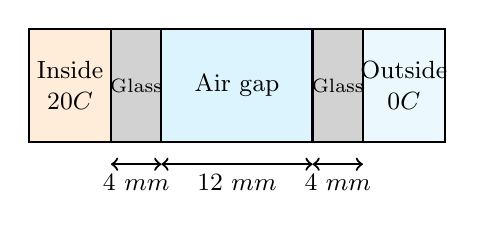
\begin{tikzpicture}[scale=0.8, font=\small]
  % Cross-section only; pane and gap widths are proportional to thickness.
  \fill[orange!15] (-1.3,0) rectangle (0,1.8);
  \fill[gray!35] (0,0) rectangle (0.8,1.8);
  \fill[cyan!14] (0.8,0) rectangle (3.2,1.8);
  \fill[gray!35] (3.2,0) rectangle (4.0,1.8);
  \fill[cyan!8] (4.0,0) rectangle (5.3,1.8);
  \draw[thick] (-1.3,0) rectangle (5.3,1.8);
  \draw[thick] (0,0) -- (0,1.8);
  \draw[thick] (0.8,0) -- (0.8,1.8);
  \draw[thick] (3.2,0) -- (3.2,1.8);
  \draw[thick] (4.0,0) -- (4.0,1.8);
  \node[align=center] at (-0.65,0.9) {Inside\\$20°\text{C}$};
  \node[align=center, font=\scriptsize] at (0.4,0.9) {Glass};
  \node[align=center] at (2.0,0.9) {Air gap};
  \node[align=center, font=\scriptsize] at (3.6,0.9) {Glass};
  \node[align=center] at (4.65,0.9) {Outside\\$0°\text{C}$};
  \draw[<->, thick] (0,-0.35) -- (0.8,-0.35)
    node[midway, below] {$4\ \text{mm}$};
  \draw[<->, thick] (0.8,-0.35) -- (3.2,-0.35)
    node[midway, below] {$12\ \text{mm}$};
  \draw[<->, thick] (3.2,-0.35) -- (4.0,-0.35)
    node[midway, below] {$4\ \text{mm}$};
\end{tikzpicture}
\end{center}
\small Cross-section schematic; layer widths are proportional to thickness.
\\[4pt]
(a) Calculate the thermal resistance of each layer:
inner glass, air gap, outer glass.\\
(b) Calculate the total thermal resistance.\\
(c) Calculate the rate of heat loss.\\
(d) Compare with a single $4\ \text{mm}$ glass pane
of the same area and temperature difference. By
what factor is the double-glazed window better?\\
(e) An alternative is to fill the gap with argon
($k_{argon} = 0.018\ \text{W\,m}^{-1}\text{K}^{-1}$).
How does this compare to the air gap version?
\hfill\ansref{Ch16-B4}

\vspace{0.4cm}

\textbf{B5.} (a) Using the Stefan-Boltzmann Law,
derive an expression for the equilibrium temperature
of a planet at distance $d$ from a star of luminosity
$L_*$ (total power output). Assume the planet has
albedo $\alpha$ (fraction of radiation reflected)
and behaves as a black body in the infrared.

(Hint: power absorbed = $(1-\alpha) \times L_*
\times \pi R_p^2 / (4\pi d^2)$; power emitted
$= \sigma \times 4\pi R_p^2 \times T^4$)\\[4pt]
(b) Use your formula to calculate the equilibrium
temperature of Mars, given:
$L_{Sun} = 3.85\times10^{26}\ \text{W}$,
$d_{Mars} = 2.28\times10^{11}\ \text{m}$,
albedo of Mars $= 0.25$.\\[4pt]
(c) The actual mean temperature of Mars is about
$-60°\text{C}$. Compare with your answer to (b)
and suggest why they may differ.\\[4pt]
(d) Using the same formula, if Earth's average
albedo increased from $0.30$ to $0.35$ due to
increased cloud cover, by how much would Earth's
equilibrium temperature change? Comment on the
direction of change and its significance.
\hfill\ansref{Ch16-B5}

\end{exercisebox}
% \end{document} % (Do not end the whole book here; main file ends the document)
